% Made up for the tikra gallery: a Riemann sum under a curve. In the playground, drag the end of
% the interval along the axis; the number of rectangles is a chip under the figure.
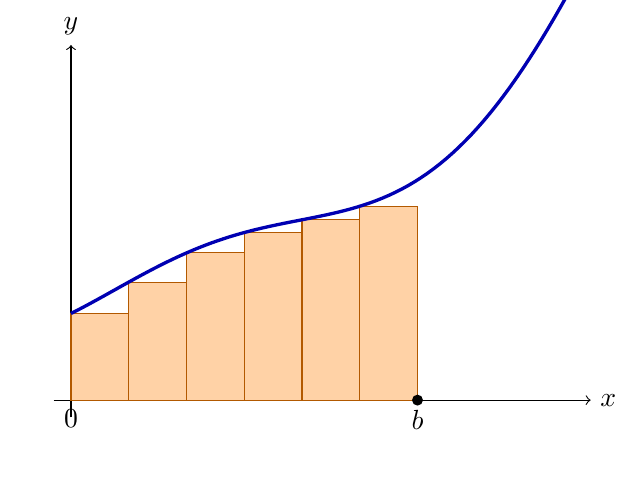
\begin{tikzpicture}[scale=1.1]
  \def\n{6}   % rectangles, 1..20
  \def\b{4}   % end of the interval, 1..5.5
  \useasboundingbox (-0.5,-0.6) rectangle (6.2,4.3);
  \draw[->] (-0.2,0) -- (6,0) node[right] {$x$};
  \draw[->] (0,-0.2) -- (0,4.1) node[above] {$y$};
  \pgfmathsetmacro\w{\b/\n}
  \foreach \i in {1,...,\n} {
    \pgfmathsetmacro\x{(\i-1)*\w}
    \pgfmathsetmacro\h{1 + 0.5*sin(deg(\x)) + 0.12*\x*\x}
    \draw[fill=orange!35, draw=orange!70!black] (\x,0) rectangle ({\x+\w},\h);
  }
  \draw[very thick, blue!70!black, domain=0:5.8, samples=80] plot (\x, {1 + 0.5*sin(deg(\x)) + 0.12*\x*\x});
  \coordinate (end) at (\b,0);
  \fill (end) circle (1.8pt) node[below] {$b$};
  \node[below] at (0,0) {$0$};
\end{tikzpicture}
